\documentclass[aspectratio=169]{beamer}
\usepackage{amsmath, amsfonts, epsfig, xspace}
\usepackage{algorithm,algorithmic}
\usepackage{pstricks,pst-node}
\usepackage{multimedia}
\usepackage[normal,tight,center]{subfigure}
\setlength{\subfigcapskip}{-.5em}
\usepackage{beamerthemesplit}
\usetheme{keynote}
\usepackage{color}
%this is for the \hl{} highlight command 
\usepackage{soul}
%This makes it able to use different colours using \hlc[colourname]{}
\newcommand{\hlc}[2][yellow]{ {\sethlcolor{#1} \hl{#2}} }
%This is for framing text
\usepackage{framed}
\definecolor{shadecolor}{RGB}{255,127,0}

%----------Customize Title--
\defbeamertemplate*{title page}{customized}[1][]
{
  \begin{shaded}
  \usebeamerfont{title}\inserttitle\par
  \end{shaded}
  %\usebeamerfont{subtitle}\usebeamercolor[fg]{subtitle}\insertsubtitle\par
  %\bigskip
  %\usebeamerfont{author}\insertauthor\par
  %\usebeamerfont{institute}\insertinstitute\par
  %\usebeamerfont{date}\insertdate\par
  \usebeamercolor[fg]{titlegraphic}\inserttitlegraphic
}

%----------Beamer Modes---
%These modes are loaded with \mode<mode name>. They may
%also appear in the <overlay specification> option in the
%\begin{frame} command or as an option to the
%\documentclass.
%\modebeamer %(default)
%\modepresentation
%\modehandout
%\modetrans %(transparencies)
%\modearticle
%\modeall
%----------Print Handouts---
%To produce handouts, change the \documentclass command to
%\documentclass[handout]{beamer} and add
%\usepackage{pgfpages} This disables hyperlinks.
%\pgfpagesuselayout{4 on 1} Puts 4 slides on each page.
%\setbeamertemplate{navigation symbols}{} Turns on
%navigation bars at the bottom of each slide.
%----------Hacks-----------------
%http://www.shawnlankton.com/2008/02/beamer-and-latex-with-keynote-theme/
%\titlegraphic{
\includegraphics[height=1cm]{iwmi}}
%\pgfdeclareimage[height=0.5cm]{iwmi}{iwmi}
%\logo{\pgfuseimage{iwmi}}
\setbeamercolor{titlelike}{parent=structure,fg=white}
%-----------------------------------

\title[European Commission\hspace{1em}\insertframenumber/\inserttotalframenumber]{\centering {Planetary Gravity Missions}}
\author[Yann CHEMIN]{Yann CHEMIN}
\institute{European Commission}
\date{} %leave out for today's date to be insterted

\begin{document}

{\usebackgroundtemplate{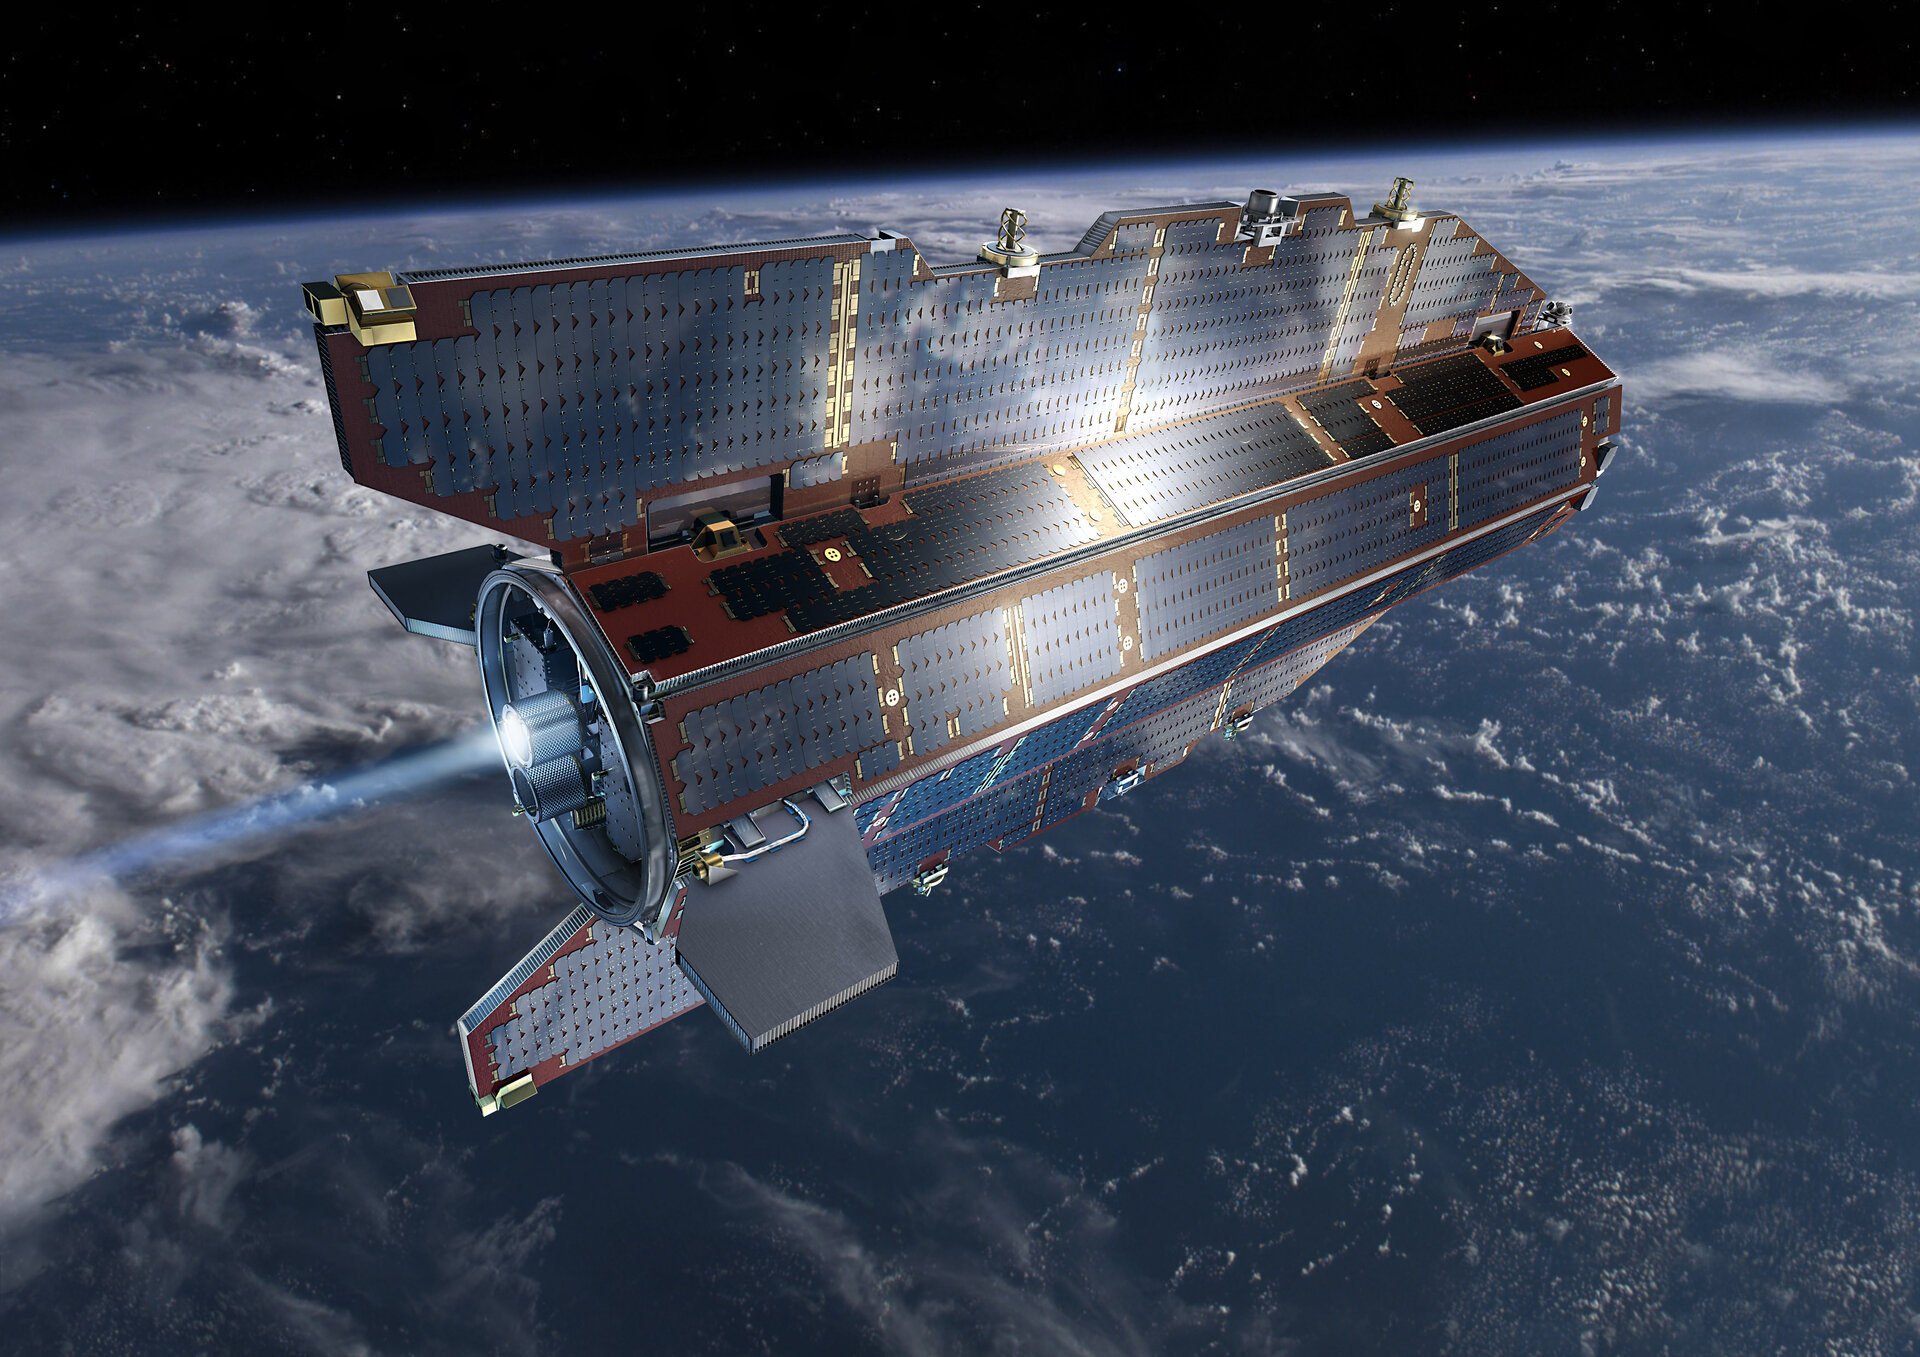
\includegraphics[height=\paperheight,width=\paperwidth]{bg_coverpage}}
\begin{frame}[plain]
\titlepage
\end{frame}}

\Large

%\begin{frame}
%  \frametitle{Processing chain}
%\begin{center}
%\begin{itemize}
% \item Fiji/ImageJ sh => Tree crowns identification NDVI-based
% \item GRASS sh => Tree crown statistics into shp file
% \item Crown Indices sh => Additional indices from refl in shp
%\end{itemize}
%\end{center}
%\end{frame}

%\transdissolve<5>
%
%\begin{frame}
%  \frametitle{GRASS script}
%\begin{center}
%\begin{itemize}
% \item GRASS7.3 in Tesla
% \item GRASS7 => RGBNIR (Acc port)
% \item GRASS7 => thermal.sh (original port)
% \item GRASS7 => rgbnir.sh (original port)
% \item \textcolor{green}{TODO: think about RGBNIR+Hyperspectral}
%\end{itemize}
%\end{center}
%\end{frame}

\transdissolve<5>

\begin{frame}
  \frametitle{Gravity Mapping from orbiting satellites}
\begin{center}
\begin{enumerate}
 \item Earth missions
	\begin{itemize}
	\item GRACE
	\item GOCE
	\end{itemize}
 \item Moon missions
	\begin{itemize}
	\item Lunar Prospector
	\item GRAIL
	\end{itemize}
\end{enumerate}
\end{center}
\end{frame}

\transdissolve<5>

{\usebackgroundtemplate{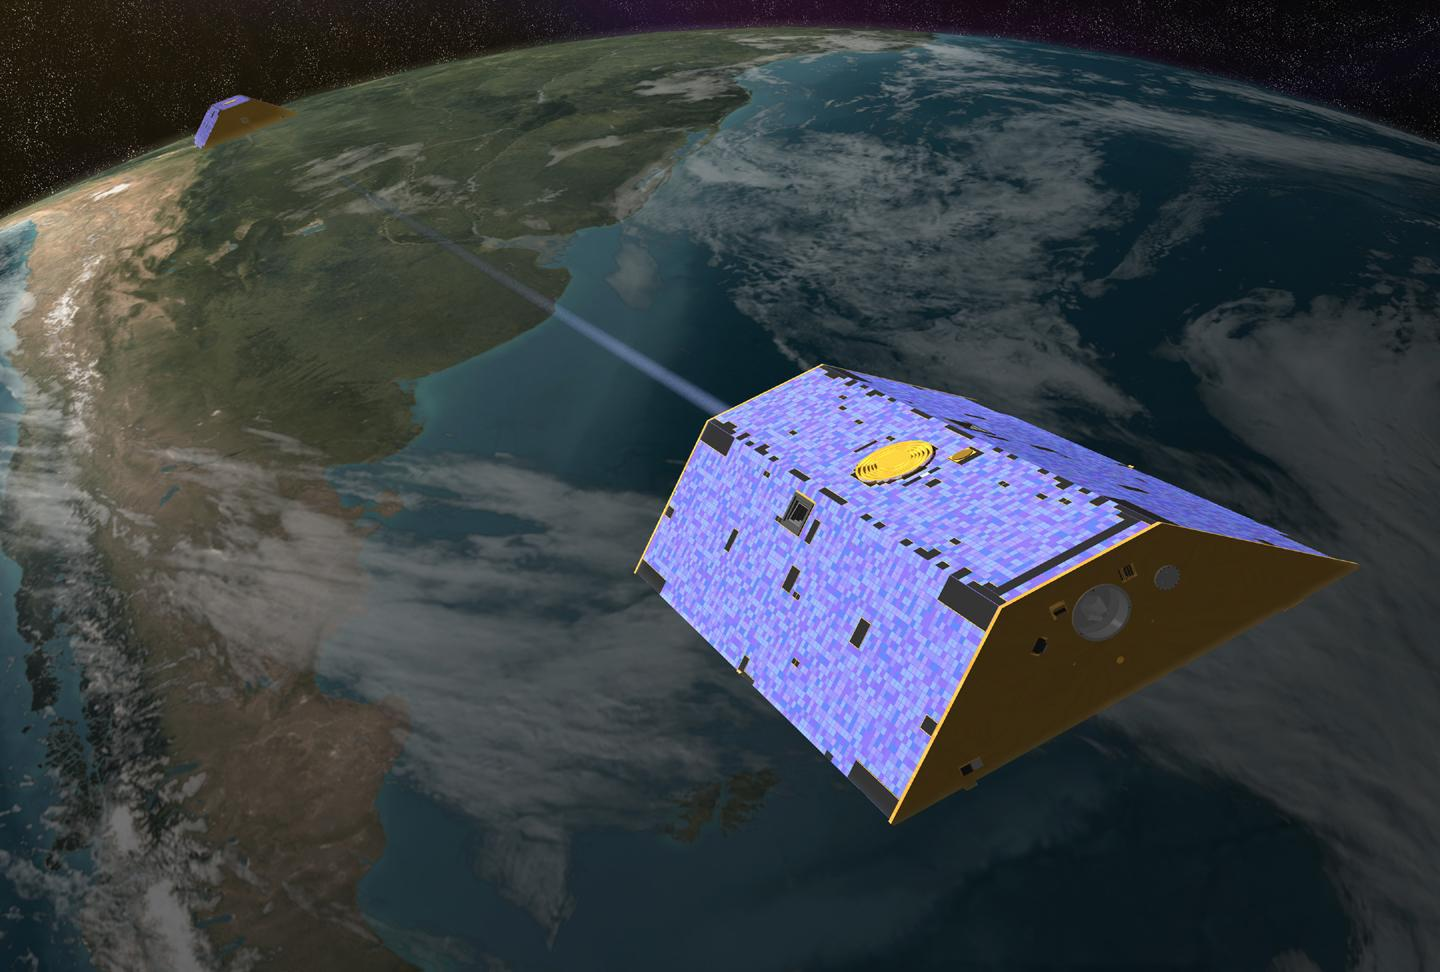
\includegraphics[height=\paperheight,width=\paperwidth]{grace.jpg}}
\begin{frame}[plain]
%\begin{shaded}
%\Huge HPC-MPI
%\end{shaded}
\end{frame}}

\transdissolve<5>

\begin{frame}
  \frametitle{1 - GRACE}
\begin{center}
\begin{itemize}
 \item Tom \& Jerry
 \item Precise measurement of changing positions and velocities
 \item Time change in mass of water, ice, solid earth 
 \item Ice sheet and ground water volume changes 
\end{itemize}
\end{center}
\end{frame}

\transdissolve<5>


{\usebackgroundtemplate{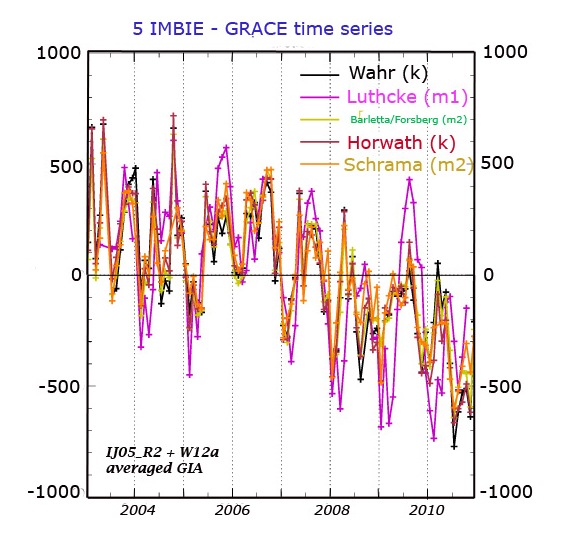
\includegraphics[height=\paperheight]{grace_gigatons_ice_loss}}
\begin{frame}[plain]
\begin{columns}[onlytextwidth]
        \begin{column}{.6\textwidth}
		%Empty for background figure
        \end{column}
	\begin{column}{0.4\textwidth}
		\begin{shaded}
			Monthly changes in Antarctic ice mass, in gigatones, as measured by NASA's Gravity Recovery and Climate Experiment (GRACE) satellites from 2003 to 2011.
		\end{shaded}
	\end{column}
    \end{columns}
\end{frame}}

\transdissolve<5>

{\usebackgroundtemplate{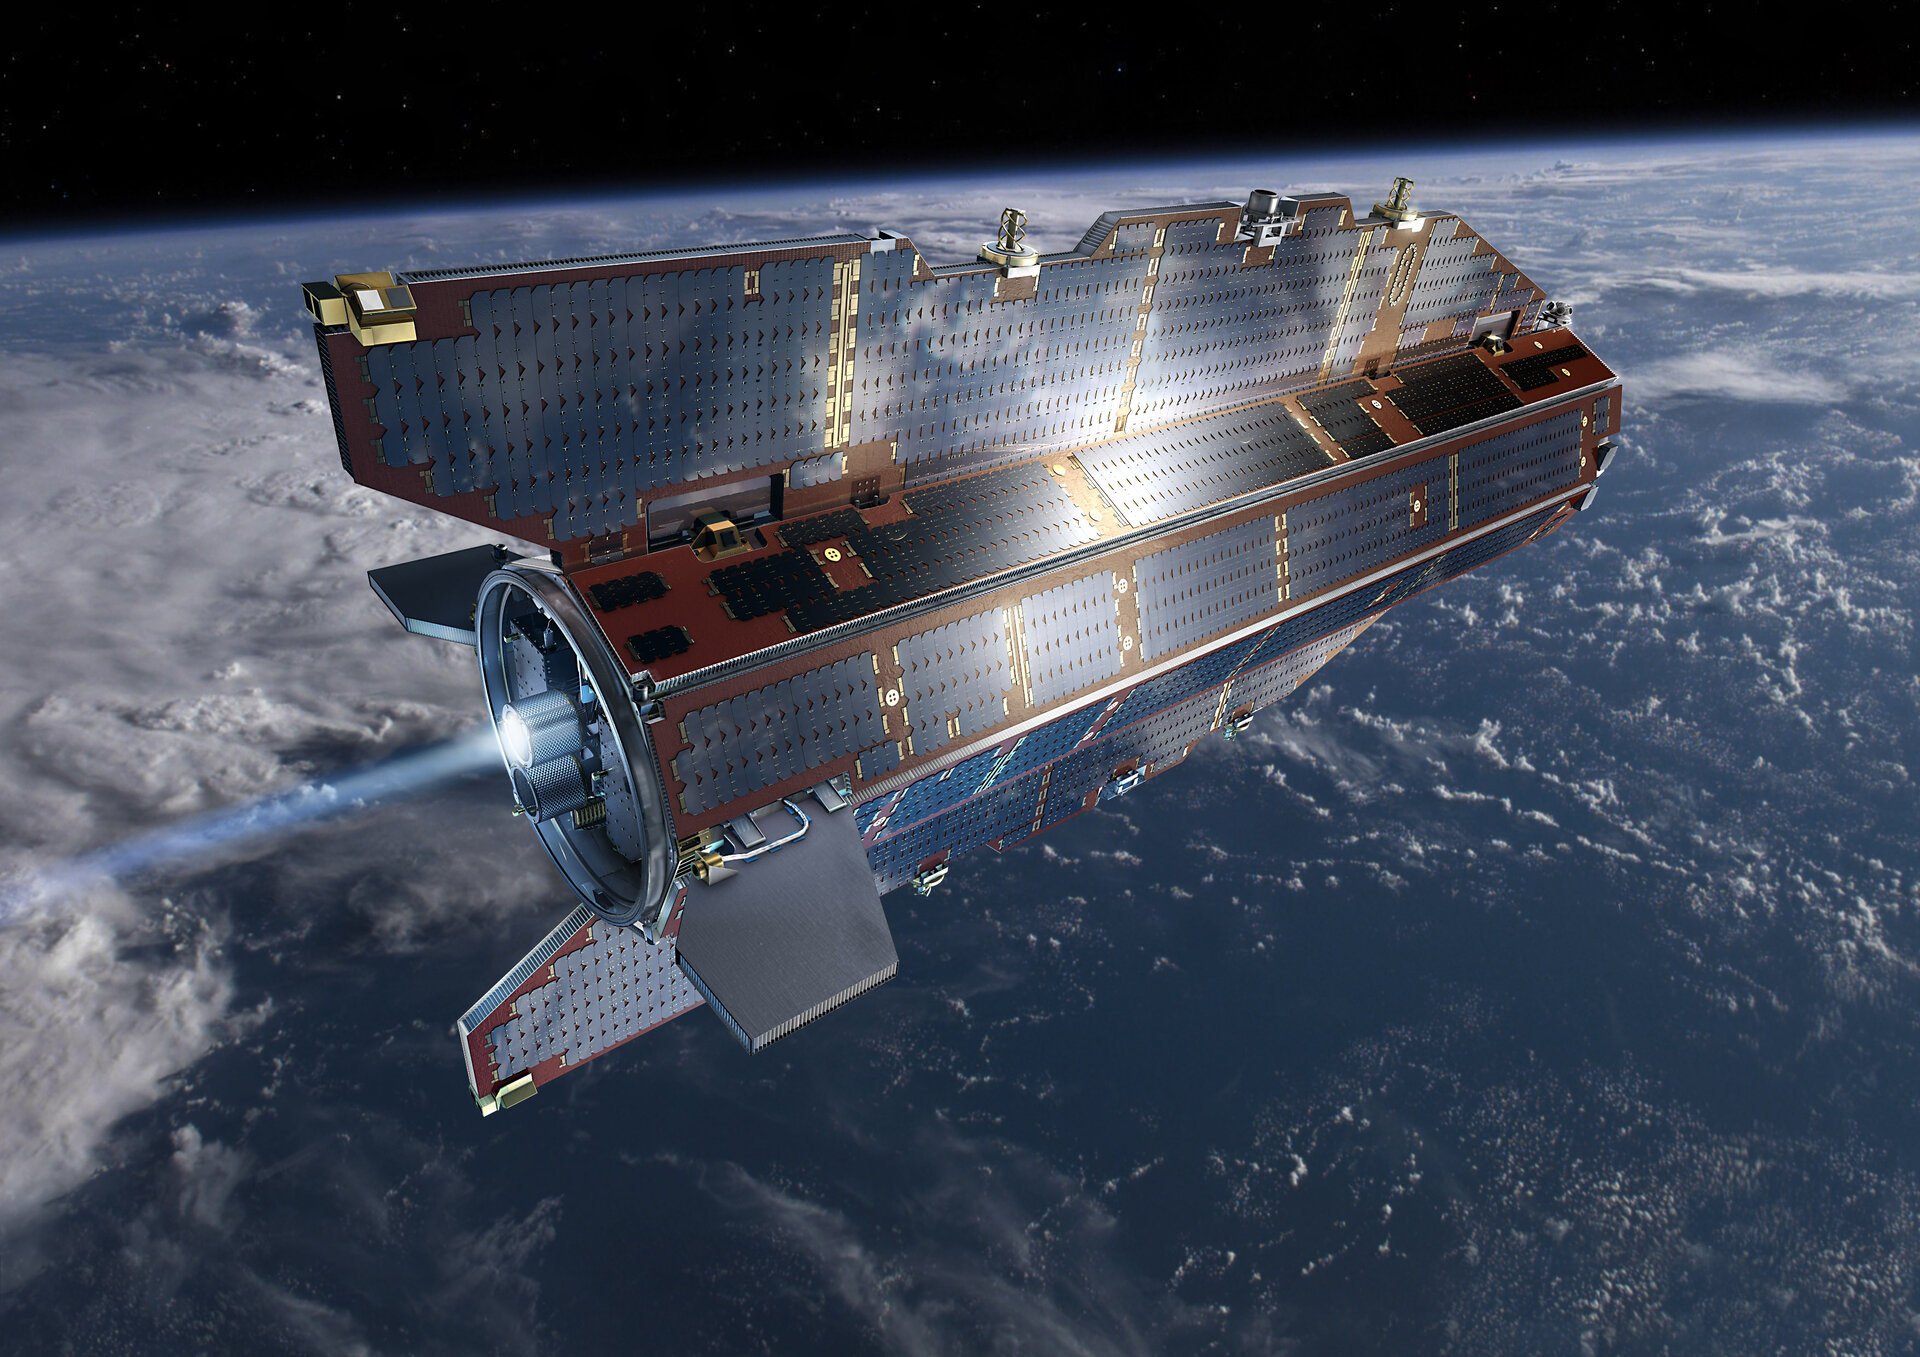
\includegraphics[height=\paperheight,width=\paperwidth]{goce}}
\begin{frame}[plain]
%\begin{shaded}
%\Huge HPC-EOSSSD
%\end{shaded}
\end{frame}}

\transdissolve<5>

\begin{frame}
  \frametitle{2 - GOCE}
\begin{center}
\begin{itemize}
 \item Oceanography, solid Earth physics, geodesy and sea-level research
 \item Mapped the best geoid of Earth so far
 \item 2009-2013
\end{itemize}
\end{center}
\end{frame}

\transdissolve<5>

{\usebackgroundtemplate{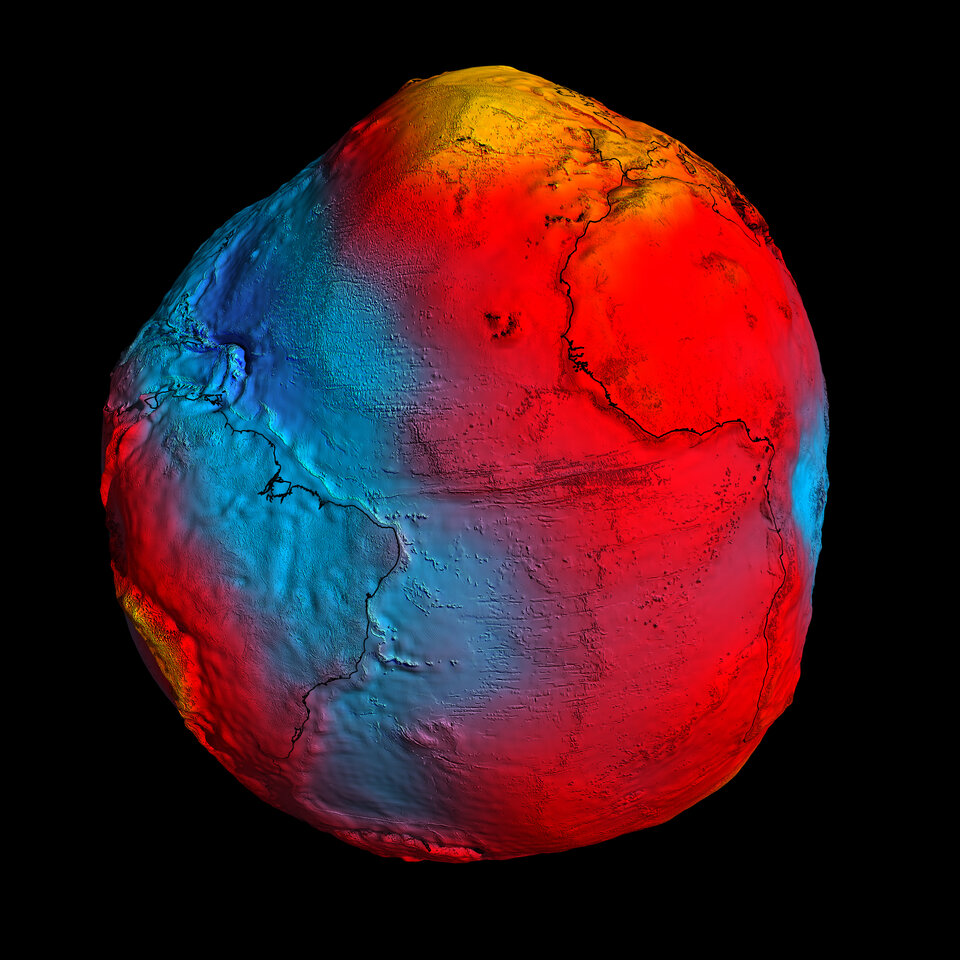
\includegraphics[height=\paperheight,width=0.7\paperwidth]{goce_geoid}}
\begin{frame}[plain]
\begin{columns}[onlytextwidth]
        \begin{column}{.7\textwidth}
		%Empty for background figure
        \end{column}
	\begin{column}{0.3\textwidth}
		\begin{shaded}
			Earth geoid
		\end{shaded}
	\end{column}
    \end{columns}
\end{frame}}

\transdissolve<5>

{\usebackgroundtemplate{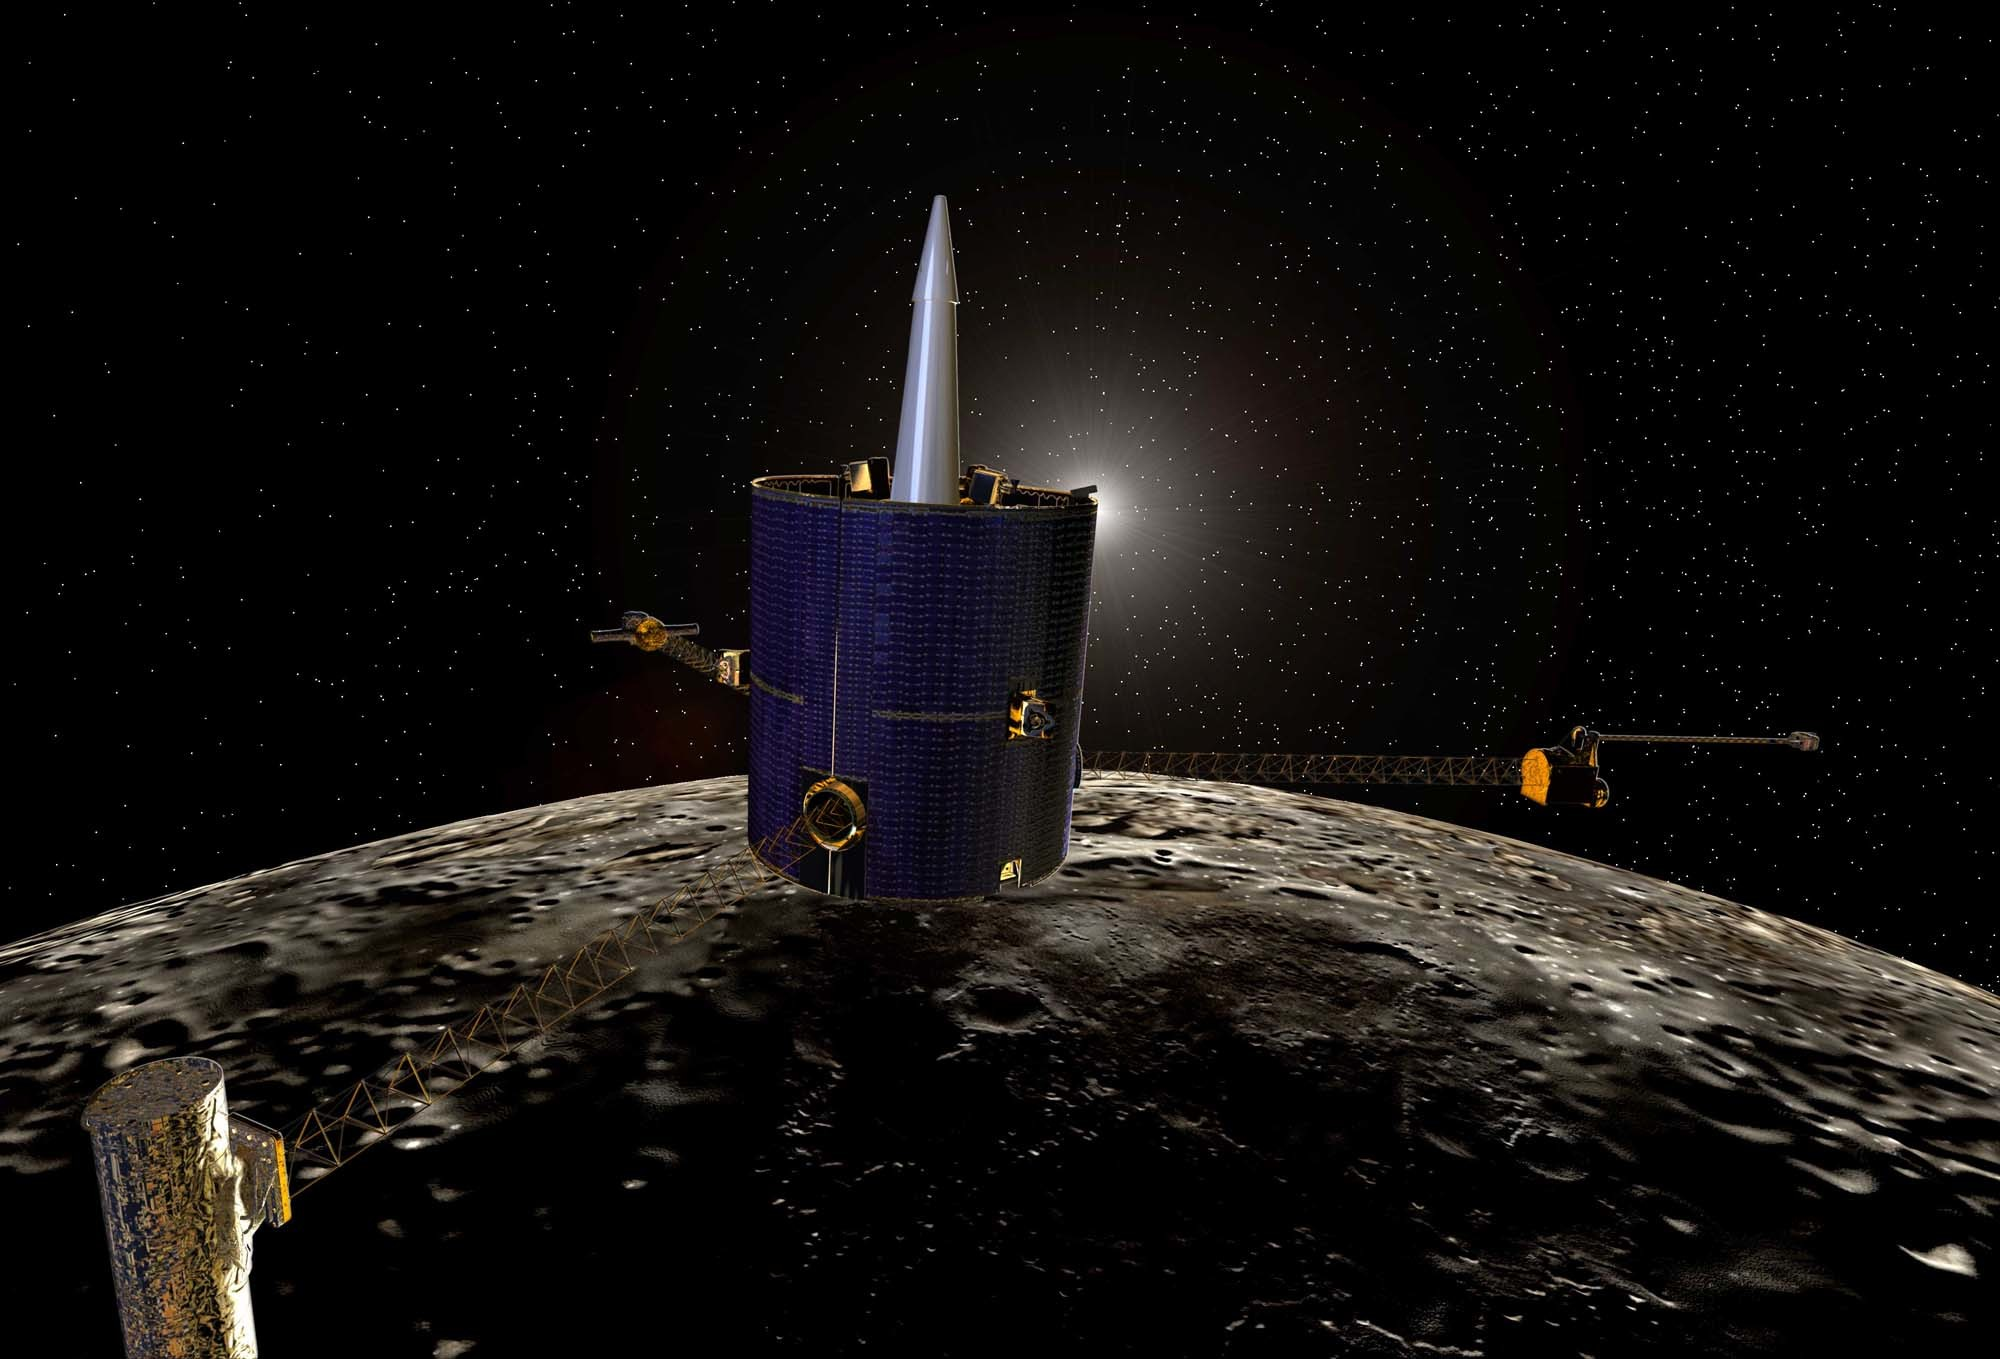
\includegraphics[height=\paperheight,width=\paperwidth]{lunar_prospector_mission}}
\begin{frame}[plain]
%\begin{shaded}
%\Huge HPC-EOSSSD
%\end{shaded}
\end{frame}}

\transdissolve<5>

\begin{frame}
  \frametitle{3 - Lunar Prospector}
\begin{center}
\begin{itemize}
 \item Multi-mission (1999-2003) 
 \item Found water ice in the Moon poles
 \item Mapped the gravity of the Moon
\end{itemize}
\end{center}
\end{frame}

\transdissolve<5>

{\usebackgroundtemplate{\includegraphics[height=\paperheight,width=\paperwidth]{lunar_prospector_mission_gravity_map}}
\begin{frame}[plain]
%\begin{shaded}
%\Huge HPC-EOSSSD
%\end{shaded}
\end{frame}}

\transdissolve<5>

{\usebackgroundtemplate{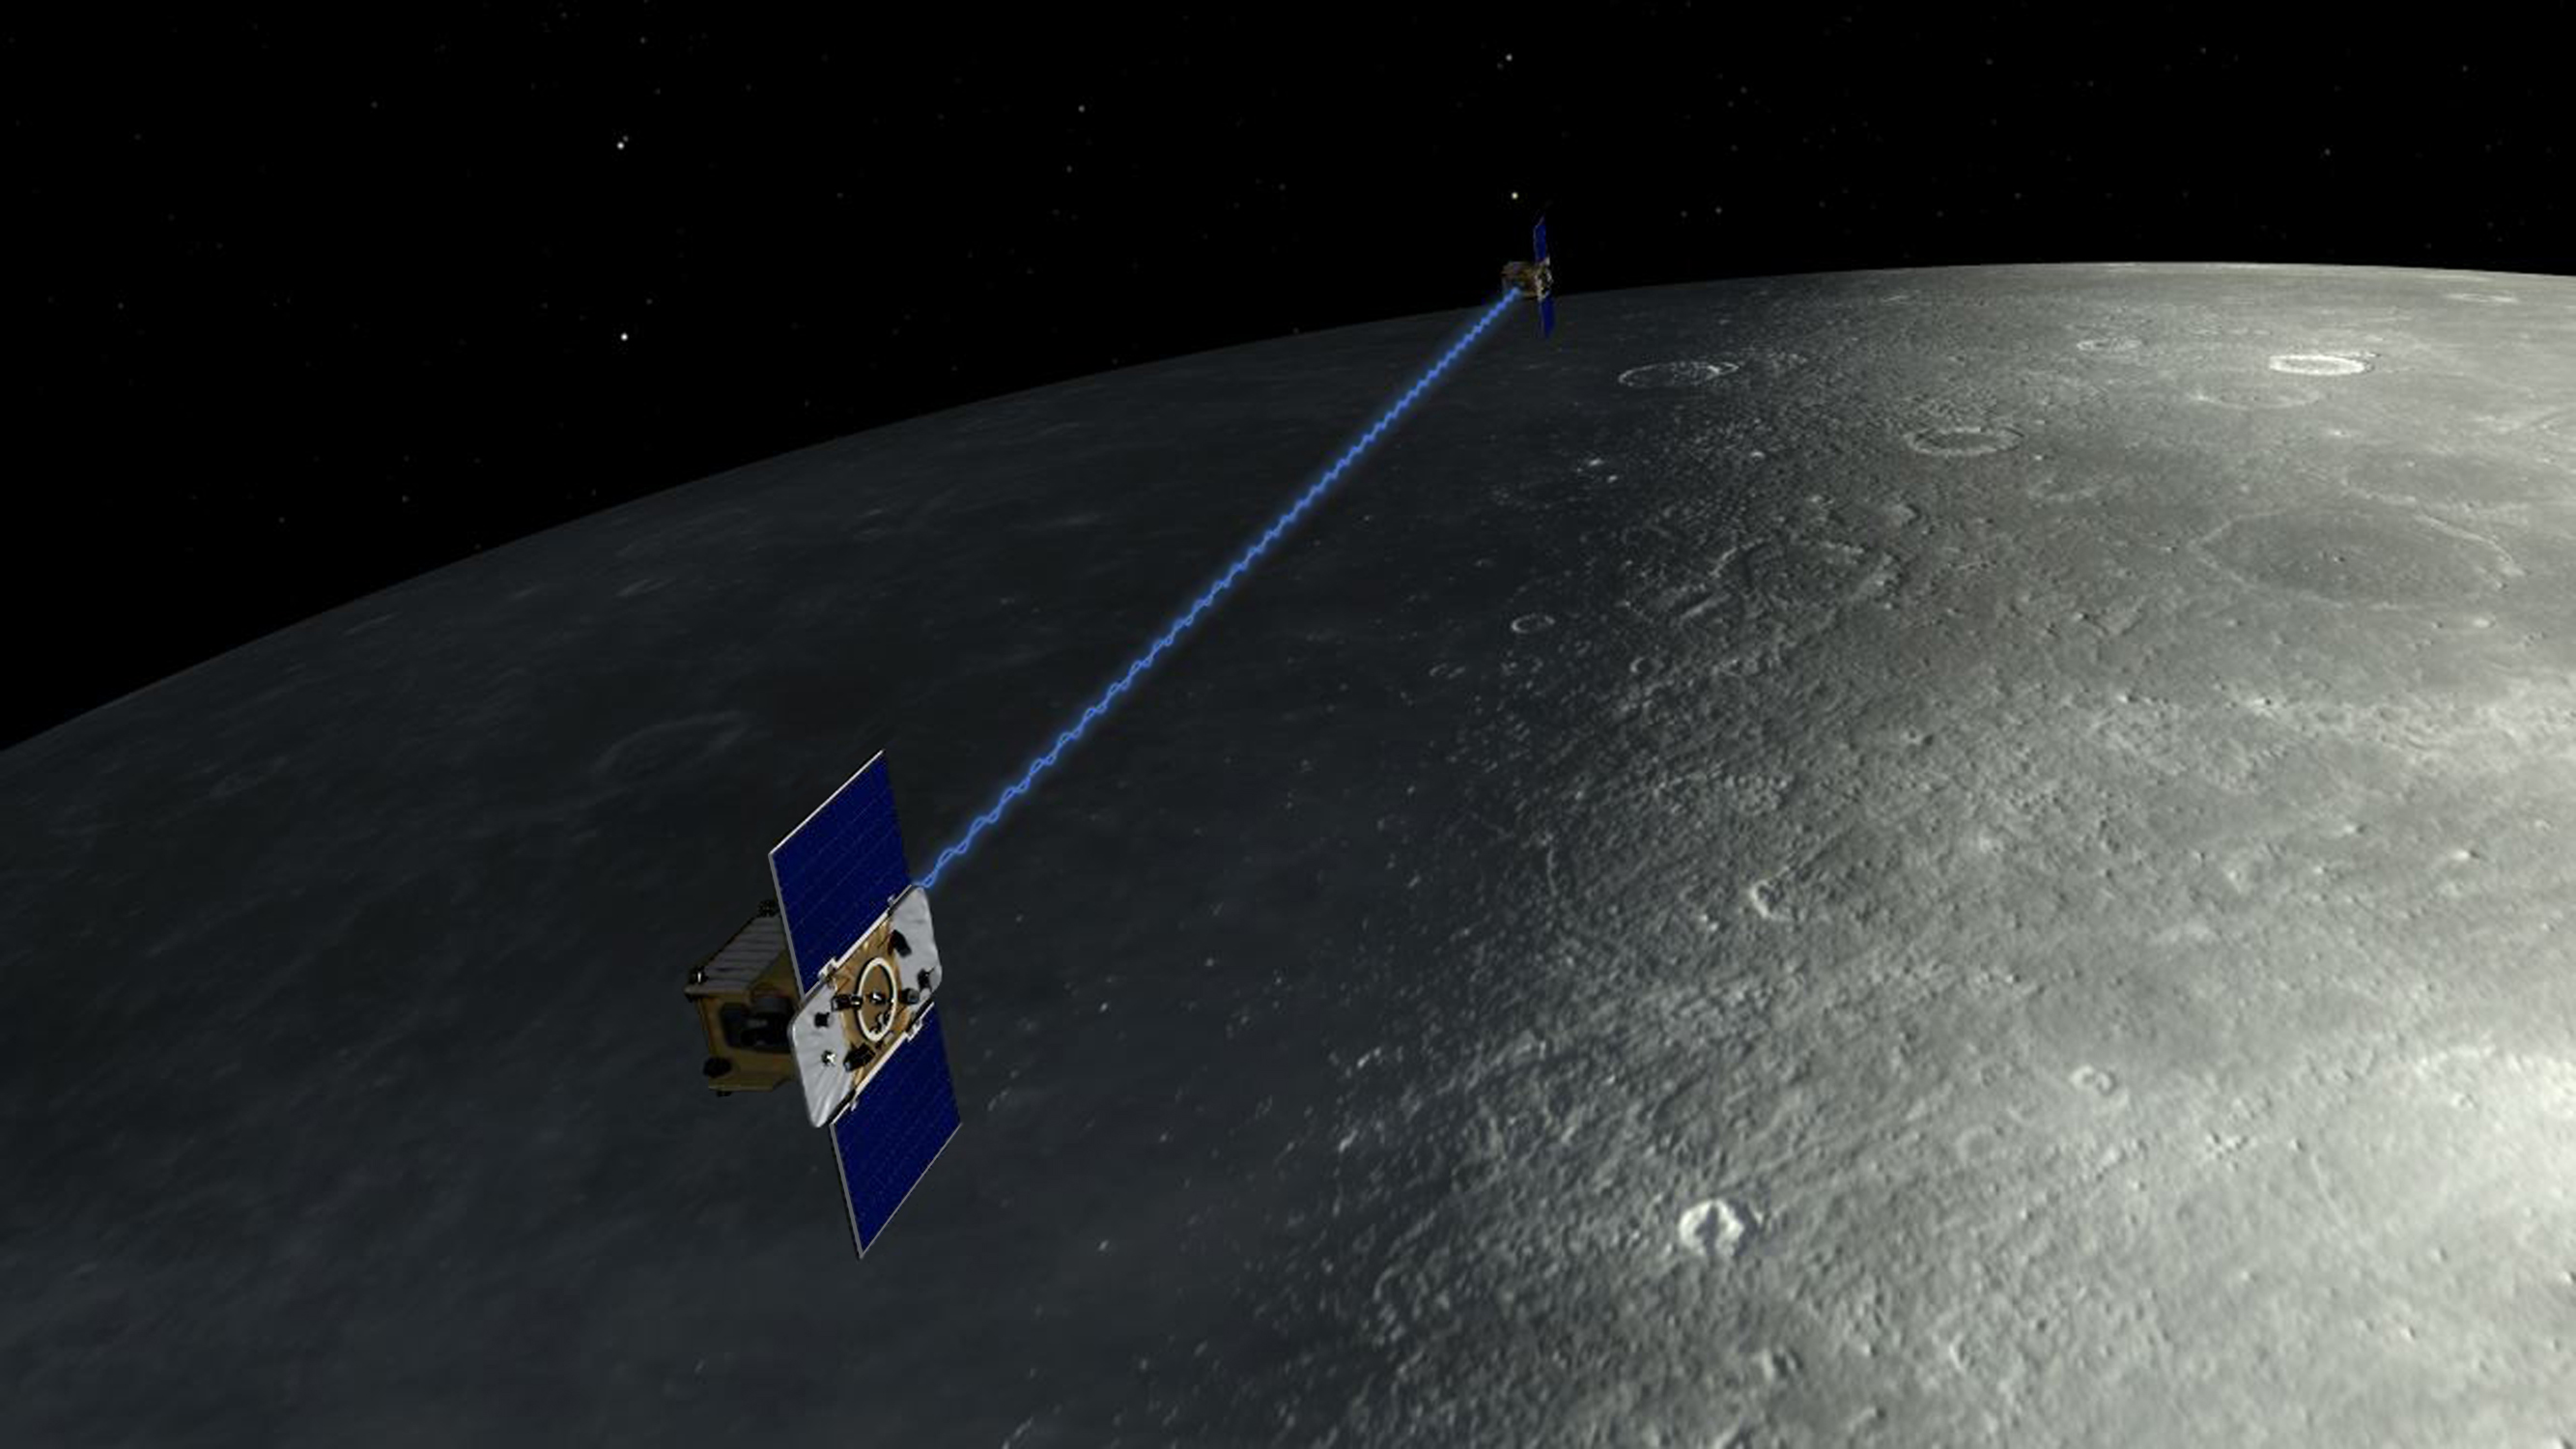
\includegraphics[height=\paperheight,width=\paperwidth]{grail}}
\begin{frame}[plain]
%\begin{shaded}
%\Huge HPC-EOSSSD
%\end{shaded}
\end{frame}}

\transdissolve<5>

\begin{frame}
  \frametitle{4 - GRAIL}
\begin{center}
\begin{itemize}
 \item Ebb \& Flow 
 \item Absence of atmosphere on the Moon
 \item Polar orbits, then concentric (declining) orbits, impact 
 \item Mapped gravity better than what was possible on Earth
\end{itemize}
\end{center}
\end{frame}

\transdissolve<5>

{\usebackgroundtemplate{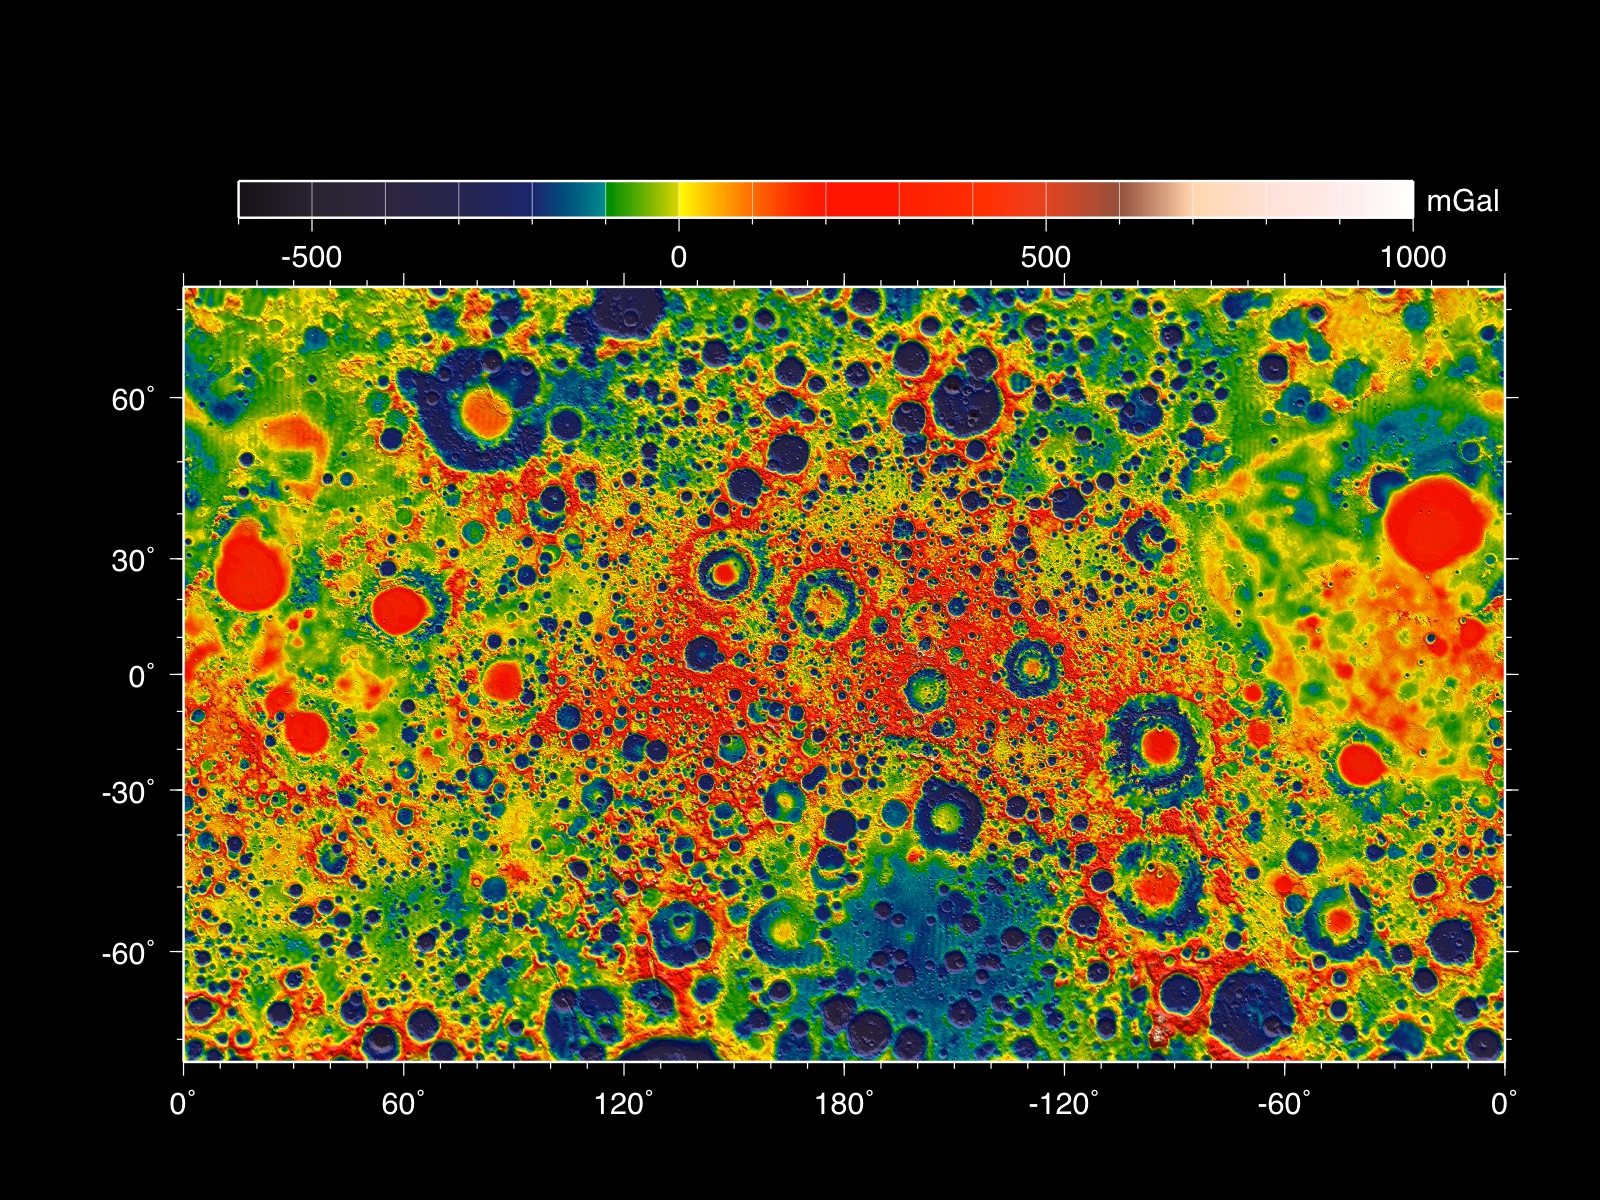
\includegraphics[height=\paperheight,width=\paperwidth]{grail_gravity_map}}
\begin{frame}[plain]
%\begin{shaded}
%\Huge HPC-EOSSSD
%\end{shaded}
\end{frame}}

\transdissolve<5>

{\usebackgroundtemplate{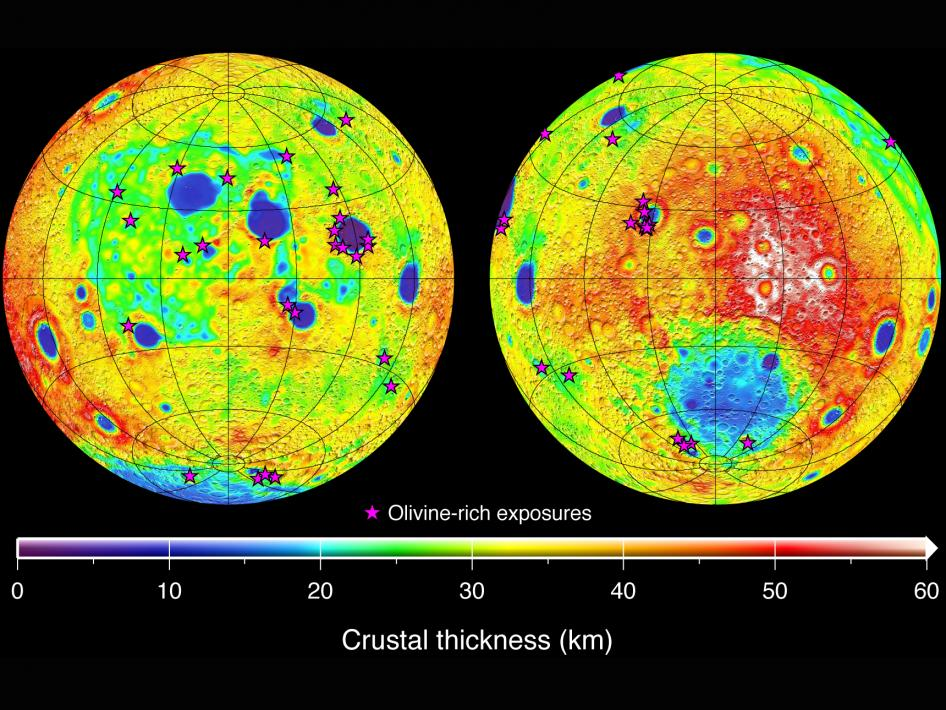
\includegraphics[height=\paperheight,width=\paperwidth]{grail_crustal_thickness}}
\begin{frame}[plain]
%\begin{shaded}
%\Huge HPC-EOSSSD
%\end{shaded}
\end{frame}}

\transdissolve<5>


%\begin{frame}
%  \frametitle{Water Level Virtual Gauge}
%\begin{columns}
%\column{0.45\textwidth}
%\begin{center}
%\begin{itemize}
 %\item Landsat Imagery
 %\item Water line
 %\item 12cm V. accuracy
 %\item 10-700Km2
 %\item Next: \\Orbital Altimetry 
%\end{itemize}
%\end{center}
%
%\column{0.5\textwidth}
%\begin{center}
% 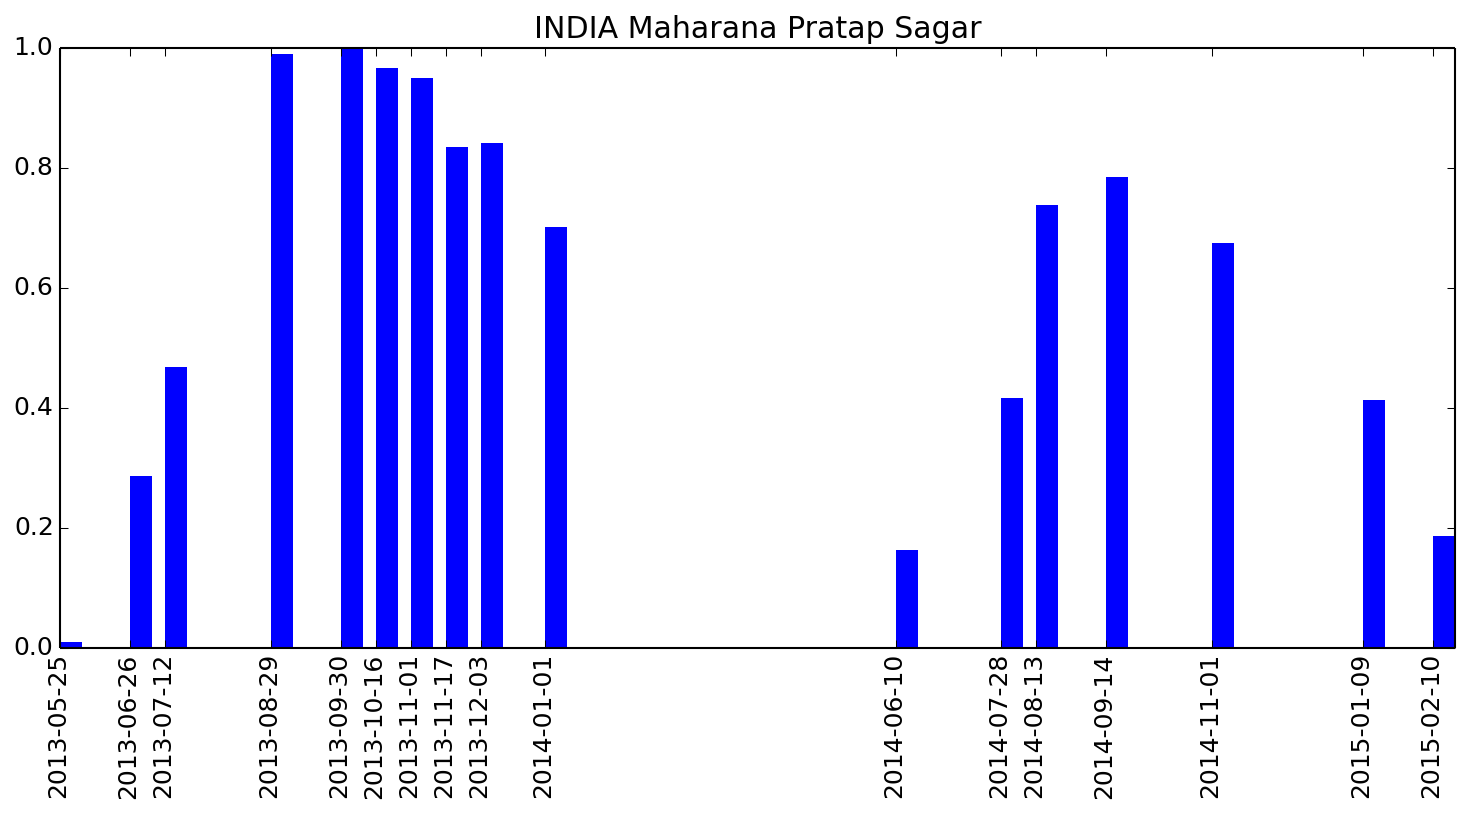
\includegraphics[height=3cm]{IN_Maharana_Pratap_Sagar_wLVG1}
% %\includegraphics[height=2.5cm]{PK_TarbelaDam_wLVG1)\\
% %\includegraphics[height=3cm]{EG_AswanDam}
%\end{center}
%\end{columns}
%\end{frame}

%\transdissolve<5>

%\begin{frame}
%  \frametitle{Equations}
%  Equations are easy
%  \begin{itemize}
%  \item Just copy and paste equations\pause
%  \item From the paper!
%    \begin{equation*}
%      \textbf{p}^* = \underset{\textbf{p}}{\arg\!\min}~\sum_{\textbf{x}}\left[ I(\textbf{W}(\textbf{x};\textbf{p})) - T(\textbf{x}) \right]^2
%    \end{equation*}
%  \end{itemize}
%\end{frame}
%
%\transdissolve<5>

%\begin{frame}
%  \frametitle{A Movie}
%  \begin{center}
%    \movie[height=5cm,width=6.5cm,poster,autostart,loop]{}{video1.avi}
%  \end{center}
%  \begin{itemize}
%  \item Movies only seem to work in Adobe Reader
%  \item Movie file is not embedded, it must be on the computer
%  \end{itemize}
%\end{frame}

%\transdissolve<5>

{\usebackgroundtemplate{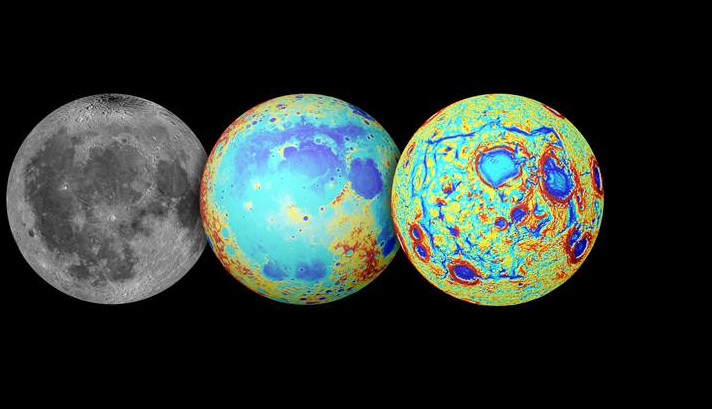
\includegraphics[height=\paperheight,width=\paperwidth]{grail_triptic}}
\begin{frame}[plain]
\begin{columns}%[onlytextwidth]
        \begin{column}{.82\textwidth}
		%Empty for background figure
        \end{column}
	\begin{column}{0.18\textwidth}
		\begin{shaded}
			Thank you
		\end{shaded}
	\end{column}
    \end{columns}
\end{frame}}
\end{document}
